\chapter{QAbstractItemModel}

QAbstractItemModel类为项模型类提供了抽象接口。\href{https://github.com/JackLovel/QtDocumentCN/blob/master/Src/A/QAbstractItemModel}{更多...} 

\begin{tabular}{|r|l|}
	\hline
	属性 & 方法 \\
	\hline
	头文件 & \#include <QAbstractItemModel>\\      
	\hline
	qmake & QT+=core\\      
	\hline
	自从 & Qt 4.6\\
	\hline
	继承&QObject \\
	\hline
	派生 & \makecell{QAbstractListModel、QAbstractProxyModel、
           QAbstractTableModel、\\QConcatenateTablesProxyModel、QDirModel、QFileSystemModel \\和 QStandardItemModel} \\
	\hline
\end{tabular}

\splitLine

公有成员类型

\begin{tabular}{|r|l|}
	\hline
	类型 & 类型名称 \\
	\hline
enum class&	CheckIndexOption{ NoOption, IndexIsValid,
  DoNotUseParent, ParentIsInvalid}\\
\hline
flags&	CheckIndexOptions\\
\hline
enum&	LayoutChangeHint { NoLayoutChangeHint, VerticalSortHint, HorizontalSortHint }\\
\hline
\end{tabular}


\splitLine

公共成员函数

\begin{longtable}{|r|l|}
\hline
类型 & 函数名称 \\
\hline
& QAbstractItemModel(QObject *parent = nullptr)\\
\hline
virtual	& $\sim$QAbstractItemModel()\\
\hline
virtual QModelIndex	& buddy(const QModelIndex \&index) const\\
\hline
virtual bool & canDropMimeData(const QMimeData *data, Qt::DropAction
               action, int row, int column, const QModelIndex
               \&parent) const s\\
\hline
virtual bool &canFetchMore(const QModelIndex \&parent) const\\
\hline
bool & checkIndex(const QModelIndex \&index,
       QAbstractItemModel::CheckIndexOptions options =
       CheckIndexOption::NoOption) const\\
\hline
virtual int&columnCount(const QModelIndex \&parent = QModelIndex())
             const = 0\\
\hline
virtual QVariant&	data(const QModelIndex \&index, int role = Qt::DisplayRole) const = 0\\
\hline
virtual bool&	dropMimeData(const QMimeData *data, Qt::DropAction
              action, int row, int column, const QModelIndex \&parent)\\
\hline
virtual void&	fetchMore(const QModelIndex \&parent)\\
\hline
virtual Qt::ItemFlags&	flags(const QModelIndex \&index) const\\
\hline
virtual bool&	hasChildren QModelIndex \&parent = QModelIndex()) const\\
\hline
bool	&hasIndex row, int column, const QModelIndex \&parent = QModelIndex()) const\\
\hline
virtual QVariant	&headerData section, Qt::Orientation orientation, int role = Qt::DisplayRole) const\\
\hline
virtual QModelIndex& index row, int column, const QModelIndex \&parent = QModelIndex()) const = 0\\
\hline
bool	&insertColumn column, const QModelIndex \&parent = QModelIndex())\\
\hline
virtual bool & insertColumns column, int count, const QModelIndex \&parent = QModelIndex())\\
\hline
bool&	insertRow(int row, const QModelIndex \&parent = QModelIndex())\\
\hline
virtual bool&	insertRows row, int count, const QModelIndex \&parent
              = QModelIndex())\\
\hline
virtual QMap<int, QVariant>	&itemData QModelIndex \&index) const\\
\hline
virtual QModelIndexList	& match QModelIndex \&start, int role, const QVariant \&value, int hits = 1, Qt::MatchFlags flags = Qt::MatchFlags (Qt::MatchStartsWith\\
\hline
virtual QMimeData *	&mimeData QModelIndexList \&indexes) const\\
\hline
virtual QStringList	& mimeTypes const\\
\hline
bool	&moveColumn QModelIndex \&sourceParent, int sourceColumn,
       const QModelIndex \&destinationParent, int destinationChild)\\
\hline
virtual bool & moveColumns QModelIndex \&sourceParent, int
               sourceColumn, int count, const QModelIndex
               \&destinationParent, int destinationChild)\\
\hline
bool& moveRow QModelIndex \&sourceParent, int sourceRow, const QModelIndex \&destinationParent, int d
estinationChild)\\
\hline
virtual bool &moveRows QModelIndex \&sourceParent, int sourceRow, int destinationChild)\\
\hline
bool &moveRow QModelIndex \&sourceParent, int sourceRow, 
       const QModelIndex \&destinationParent, 
       int destinationChild)\\    
\hline           
virtual bool &moveRows QModelIndex \&sourceParent, int sourceRow, 
               int count, const QModelIndex \&destinationParent, int destinationChild)\\
\hline
virtual QModelIndex&	parent QModelIndex \&index) const = 0\\
\hline
bool&	removeColumn column, const QModelIndex \&parent = QModelIndex())\\
\hline
virtual bool&	removeColumns column, int count, const QModelIndex \&parent = QModelIndex())\\
\hline
bool&	removeRow row, const QModelIndex \&parent = QModelIndex())\\
\hline
virtual bool&	removeRows row, int count, const QModelIndex \&parent = QModelIndex())\\
\hline
virtual QHash<int, QByteArray>&	roleNames const\\
\hline
virtual int	& rowCount QModelIndex \&parent = QModelIndex()) const = 0\\
\hline
virtual bool &setData QModelIndex \&index, const QVariant \&value, int role = Qt::EditRole)\\
\hline
virtual bool	&setHeaderData section, Qt::Orientation orientation, const QVariant \&value, int role = Qt::EditRole)\\
\hline
virtual bool	&setItemData QModelIndex \&index, const QMap<int, QVariant> \&roles)\\
\hline
virtual QModelIndex&	sibling row, int column, const QModelIndex \&index) const\\
\hline
virtual void	&sort column, Qt::SortOrder order = Qt::AscendingOrder)\\
\hline
virtual QSize	&span QModelIndex \&index) const\\
\hline
virtual Qt::DropActions	&supportedDragActions const\\
\hline
virtual Qt::DropActions	&supportedDropActions const\\
\hline
\end{longtable}

\splitLine

公共槽函数

\begin{tabular}{|r|l|}
\hline
类型 & 函数名称 \\
\hline
virtual void	&revert()\\
\hline
virtual bool	&submit()\\
\hline
\end{tabular}

\splitLine

信号

\begin{tabular}{|r|l|}
\hline
类型 & 函数名称 \\
\hline
void&	columnsAboutToBeInserted QModelIndex \&parent, int first, int last)\\
\hline
void&	columnsAboutToBeMoved(const QModelIndex \&sourceParent, int sourceStart, int sourceEnd, const QModelIndex \&destinationParent, int destinationColumn)\\
\hline
void&	columnsAboutToBeRemoved(const QModelIndex \&parent, int first, int last)\\
\hline
void&	columnsInserted(QModelIndex \&parent, int first, int last)\\
\hline
void&	columnsMoved(const QModelIndex \&parent, int start, int end, const QModelIndex \&destination, int column)\\
\hline
void&	columnsRemoved(const QModelIndex \&parent, int first, int last)\\
\hline
void&	dataChanged(const QModelIndex \&topLeft, const QModelIndex \&bottomRight, const QVector \&roles = QVector())\\
\hline
void&	headerDataChanged(Qt::Orientation orientation, int first, int last)\\
\hline
void&	layoutAboutToBeChanged(const QList \&parents = QList(), QAbstractItemModel::LayoutChangeHint hint = QAbstractItemModel::NoLayoutChangeHint)\\
\hline
void&	layoutChanged(const QList \&parents = QList(),
      QAbstractItemModel::LayoutChangeHint hint = QA
bstractItemModel::NoLayoutChangeHint)\\
\hline
void&	modelAboutToBeReset()\\
\hline
void&	modelReset()\\
\hline
void&	rowsAboutToBeInserted(const QModelIndex \&parent, int start, int end)\\
\hline
void&	rowsAboutToBeMoved(const QModelInd
ex \&sourceParent, int
      sourceStart, int sourceEnd, const QM
odelIndex \&destinationParent, int destinationRow)\\
\hline
void&	rowsAboutToBeRemoved(const QModelIndex \&parent, int first, int last)\\
\hline
void&	rowsInserted(const QModelIndex \&parent, int first, int last)\\
\hline
void&rowsMoved(const QModelIndex \&parent, int start, 
  int end, const QModelIndex \&destination, int row) \\
\hline
void&	rowsRemoved(const QModelIndex \&parent, int first, int last)\\
\hline
\end{tabular}

\splitLine

受保护的函数

\begin{tabular}{|r|l|}
\hline
类型 &	 函数名称\\
\hline
void&	beginInsertColumns(const QModelIndex \&parent, int first, int
      last)\\
\hline
void&	beginInsertRows(const QModelIndex \&parent, int first, int
      last)\\
\hline
bool&	beginMoveColumns(const QModelIndex \&sourceParent, int
  sourceFirst, int sourceLast, const QModelIndex \&destinationParent,
  int destinationChild)\\
\hline
bool&	beginMoveRows(const QModelIndex \&sourceParent, int
      sourceFirst, int sourceLast, const QModelIndex
      \&destinationParent, int destinationChild)\\
\hline
void&	beginRemoveColumns(const QModelIndex \&parent, int first, int
      last)\\
\hline
void&	beginRemoveRows(const QModelIndex \&parent, int first, int last)\\
\hline
void&	beginResetModel()\\
\hline
void&	changePersistentIndex(const QModelIndex \&from, const QModelIndex \&to)\\
\hline
void&	changePersistentIndexList(const QModelIndexList \&from, const
   QModelIndexList \&to)\\
\hline
QModelIndex&	createIndex(int row, int column, void *ptr = nullptr) const\\
\hline
QModelIndex&	createIndex(int row, int column, quintptr id) const\\
\hline
void&	endInsertColumns()\\
\hline
void&	endInsertRows()\\
\hline
void&	endMoveColumns()\\
\hline
void&	endMoveRows()\\
\hline
void&	endRemoveColumns()\\
\hline
void&	endRemoveRows()\\
\hline
void&	endResetModel()\\
\hline
QModelIndexList&	persistentIndexList() const\\
\hline
\end{tabular}

受保护的槽函数

\splitLine

\begin{tabular}{|r|l|}
\hline
类型 	&函数名称\\
\hline
void	&resetInternalData()\\
\hline
\end{tabular}

详细描述

\splitLine

QAbstractItemModel 类定义了项模型与模型/视图体系结构中的其他组件进行交互操作时必须使用的标准接口。应该子类化该类创建新的模型,而不是直接实例化使用。

QAbstractItemModel 类是模型/视图类中的一个,也是 Qt 模型/视图框架的一部分。它可以用作 QML 中的项视图元素或 Qt Widgets 模块中的项视图类的底层数据模型。

如果需要一个模型来使用项视图,比如 QML 的 List View 元素或者 C++ widgets 的 QListView 或者  QTableView,应该考虑子类化 QAbstractListModel 或者 QAbstractTableModel 而不是使用该类。

底层数据模型作为表的层次结构暴露给视图和委托。如果不使用层次结构,那么模型就是一个简单的具有行和列的表。每个项都有一个由 QModelIndex 指定的惟一索引。

\begin{figure}[hbt!]  
	\centering
    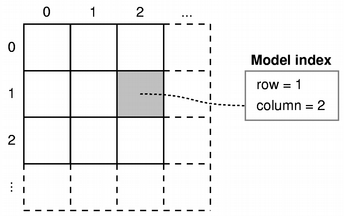
\includegraphics[width=0.5\textwidth]{modelindex-no-parent}
	\caption{model index}
\end{figure}

%%% Local Variables:
%%% mode: latex
%%% TeX-master: "../../master"
%%% End:
